\documentclass[Report.tex]{subfiles}

\newcommand{\newaxis}[4]{
\begin{axis}[
    ybar,
    title={#1},
    ymin=#3, ymax=#4,
    bar width=1em,
    legend style={at={(0.5,-0.25)},anchor=north,legend columns=-1},
    enlarge x limits=0.4,
    x tick label style={align=center,text width=1.7cm},
    symbolic x coords={Logistic Regression, Random Forest, Multi-layer Perceptron},
    xtick=data,
    ylabel={#2}
]
}
% Read data
%\newcommand{\accprerecbarplot} {
%  \addplot+[
%    discard if not={feature}{#1},
%] table [x expr=\coordindex, y={accuracy}] {};
%}

%\pgfplotstableread[col sep=comma]{data/15-pair-cv.csv}\fifteenPairCV

\begin{document}

\section{Player identification}\label{sec:game-classification}
This section describes the methodology behind the classification problem to answer the question: \textit{Given a match of Dota 2, who is the player playing this hero?} TODO 

The different experiments conducted are also detailed with the discussion and analysis of their results. 



\subsection{Approach}
To simplify the process and results, this approach took the view of looking at the question as a binary classification problem. This rephrases the question as: \textit{Given a match of Dota 2, is it player X playing this hero?} where player X is the single player to be matched on. All other players are simply considered as not player X. 

Particular attention is drawn to the exploration of the mouse movement features. While the game statistic and itemisation features output once for each match, for example total gold gained per minute, or the hashed encoding of inventory items is only output as one sample each, the mouse movement features create samples for every defined level 3 mouse action that a player makes, generating thousands of actions in a single match. As such, the exploration of mouse movement features was done in two different approaches. 

The first looked at using each action as a data point for training and testing. This means the context of what is a match is lost and it becomes a classification problem of individual mouse actions rather than a classification of matches. By encoding the data this way, a large number of training and testing samples were created, as all the actions were concatenated together. The results of this approach give an indication to how useful individual actions are, and whether they can be used, or if further processing, such as grouping the actions into time slices was required or not. The second approach grouped all mouse movement features of a single match together, which is representative of the classification problem of Dota 2 matches. 

% Each action was then tagged as one of two groups - is the player or is not the player. In this binary classification problem, only a single player is trained as one group and all other players as the other group. In this sense, the question being asked becomes \textit{given a level 3 action, is the player who performed this action player X?} Moreover, by encoding the data this way, a large number of training and testing samples are created from just a small number of games, as each game contained thousands of level 3 actions.

% The models therefore are training on each row and predicted whether a single action belonged to the player or not.

% In the second iteration, the mouse movement features are grouped together for each match. This gave the models each match as a data point, which is more representative of the problem of classifying a match of Dota 2.

\begin{figure}[H]
\pgfdeclarelayer{background}
\pgfdeclarelayer{foreground}
\pgfsetlayers{background,main,foreground}

% Block styles
\tikzstyle{data}=[draw, fill=blue!20, text width=5em, 
    text centered, minimum height=2.5em]
\tikzstyle{model} = [data, text width=5em, fill=red!20, 
    minimum height=3em, rounded corners]

\def\blockdist{3}
\newcommand{\newMoveModel}[3]{
    \node (#2-model) at (2,#3) [model] {#1 Model};
    \path (#2-model.west)+(-\blockdist,0) node (#2) [data] {#1 actions}; 
   
    \path (#2-model.east)+(\blockdist,0) node (#2-output) [data] {Predictions};
    
    \path [draw, ->] (#2.east) -- node {} (#2-model);
    \path [draw, ->] (#2-model.east) -- node{} (#2-output);
}

\newcommand{\newGameModel}[4]{
    \node (#2-model) at (2,#3) [model] {#1 Model};
    \path (#2-model.west)+(-\blockdist,0) node (#2) [data] {#4}; 
   
    \path [draw, ->] (#2.east) -- node {} (#2-model);
}
\begin{subfigure}{1\textwidth}
\centering
\begin{tikzpicture}
\newMoveModel{AC}{ac}{4}
\newMoveModel{MC}{mc}{2.5}
\newMoveModel{SC}{sc}{1}
\end{tikzpicture}
\caption{Classifying individual mouse actions}
\vspace{\baselineskip}
\end{subfigure}

\hspace{\fill}

\begin{subfigure}{1\textwidth}
\centering
\def\blockdist{2}
\begin{tikzpicture}
\newGameModel{AC}{ac}{4}{AC actions}
\newGameModel{MC}{mc}{2.5}{MC actions}
\newGameModel{SC}{sc}{1}{SC actions}
\newGameModel{Stats}{stats}{-0.5}{Game statistics}
\newGameModel{Items}{items}{-2.0}{Game items}

\path (sc-model.west)+(-6,0) node (game) [data] {Game};
\path (sc-model.east)+(2.5,0) node (combine) [model] {MLP};
\path (combine.east)+(2.5,0) node (output) [data] {Prediction};

\path [draw, ->] (game.20) -- node [above] {} (ac.180);
\path [draw, ->] (game.10) -- node [above] {} (mc.180);
\path [draw, ->] (game.0) -- node [above] {} (sc.180);
\path [draw, ->] (game.350) -- node [above] {} (stats.180);
\path [draw, ->] (game.340) -- node [above] {} (items.180);

\path [draw, ->] (ac-model.east) -- node [above] {} (combine.160);
\path [draw, ->] (mc-model.east) -- node [above] {} (combine.170);
\path [draw, ->] (sc-model.east) -- node [above] {} (combine.180);
\path [draw, ->] (stats-model.east) -- node [above] {} (combine.190);
\path [draw, ->] (items-model.east) -- node [above] {} (combine.200);

\path [draw, ->] (combine.east) -- node [above] {} (output);

\begin{pgfonlayer}{background}
  \path (ac.west |- ac.north)+(-0.5,0.5) node (a) {};
  \path (ac-model.south -| combine.east)+(+0.5,-0.5) node (b) {};
  \path (combine.east |- items-model.east)+(+0.5,-1) node (c) {};        
  \path[fill=yellow!20,rounded corners, draw=black!50, dashed] (a) rectangle (c);           
  \path (ac.north west)+(-0.2,0.2) node (a) {};        
\end{pgfonlayer}
\end{tikzpicture}
\caption{Classifying a single match}
\end{subfigure}
\caption{Difference between classifying each level 3 action and classifying each game. For the game classifier, each type of level 3 action is split per game and evaluated with separate models. This also allows new features to be easily added to the classifier in later stages. The probability of the separate models are then used for the combining model (MLP).}

\label{fig:game-classifier-difference}
\end{figure}

In order to combine the separate mouse actions from a match together, separate models were used to evaluate each type of level 3 action using the first approach. The results of the separate models are then combined by a simple multi-layer perceptron which takes the probability output of the models. The probability was chosen over the prediction to give the combining neural network a better range of values, rather than a binary output of the predicted class. The idea of using a simple network for the combination step is to be able to learn the relative weights for each type of mouse action, rather than use them all equally in a voting scheme, or set arbitrary weights to them. This does mean the network has to be trained in addition to training the separate models, but this is simply a small computational cost. Further, this approach is modular, as the addition of more features for combination can be easily added as a separate model and input into the combining network.

The combining neural network was kept very simple in order to avoid complications with large hidden layers and activation functions, as its purpose was to learn and balance weights between the different features to give the best performance. %It uses a TODO activation function and only contains one hidden layer with 3 nodes.


\subsection{Experimental design}
The features discussed in section \ref{sec:methodology} were initially explored individually to examine their performance. Where the features contained multiple approach or subtypes, such as the itemisation encoding and types of mouse actions, each was also explored individually to ascertain which approach performed better. As this approach used individual matches, the training and testing datasets were split carefully to ensure the testing set contained players and matches which do not appear in the training set, in order to eliminate potential data leakage. The one player used as the positive sample class was the only player which appeared in both training and testing sets. All the experiments used a two-step evaluation method to obtain metrics for training and testing.
\begin{enumerate}
\item During training, evaluation metrics were gathered using a 5-fold cross evaluation. This gives an idea on how well the models and feature perform, but the performance is likely inflated as the same players may appear in both the training and evaluation data. A 5-fold cross evaluation was chosen to give a balance between the amount of data used for training and evaluation (80\% and 20\% respectively for each fold) and performing enough runs to get a strong average. 
\item After the 5-fold cross evaluation, the final model is trained using all the training data, and evaluated against the testing data. This is the best indication of how the models perform against unseen data, as the testing data is untouched until this point of the experiment. 
\end{enumerate}
%Four
Three different models were used for evaluation. These models were chosen based on what was used in related work \cite{TODO} and to cover a range of different approaches. The three models are logistic regression, random forest and a neural network (in the form of a multi-layer perceptron). \cite{TODO} used logistic regression and neural networks, while \cite{TODO} use logistic regression and random forests.  TODO. 

Three performance metrics were used to evaluate the features and the machine learning models: accuracy, precision and recall. Each metric measures a different aspect of performance. 

\textbf{Accuracy} \\
Accuracy measures the overall performance of the model and feature by computing the total number of correct predictions over the total number of predictions.
\begin{equation*}
\text{accuracy} = \frac{\text{correct predictions}}{\text{total predictions}}
\end{equation*}
It is a simple measure that gives a good indication to the performance, but is relatively limited in what it can reveal. It can be inaccurate when the percentage of classes are unbalanced, as a model that predicts only the majority class will still achieve a high accuracy. Further, accuracy does not reveal additional detail about where misclassification occurs as it does not differentiate between false positives and false negatives. 

\textbf{Precision and Recall} \\
Precision and recall are complementary metrics that measure the relevance of predictions, with precision taking into account false positive results and recall taking into account false negative results. 
\begin{equation*}
\text{precision} = \frac{\text{true positives}}{\text{true positives} + \text{false positives}}
\end{equation*}

\begin{equation*}
\text{recall} = \frac{\text{true positives}}{\text{true positives} + \text{false negatives}}
\end{equation*}
In other words, precision helps identify the accuracy of positive predictions and recall helps identify the accuracy of predicting positive samples. These measures are useful to help narrow down why certain features or models may be behaving in a certain way. For example, a high recall but low precision suggests the model or feature is biased towards positive samples, as there are low false negatives but high false positives. 
\subsection{Results}

\subsubsection{Mouse movement features}\label{sec:mm-features-results}
The three types of level 3 mouse actions (MMAC, MMMC and MMSC) described in section \ref{sec:mm-features} are first evaluated separately with the different models.

\subsubsection{Individual mouse actions}
 
\begin{figure}[H]
\begin{subfigure}{1\textwidth}
\centering
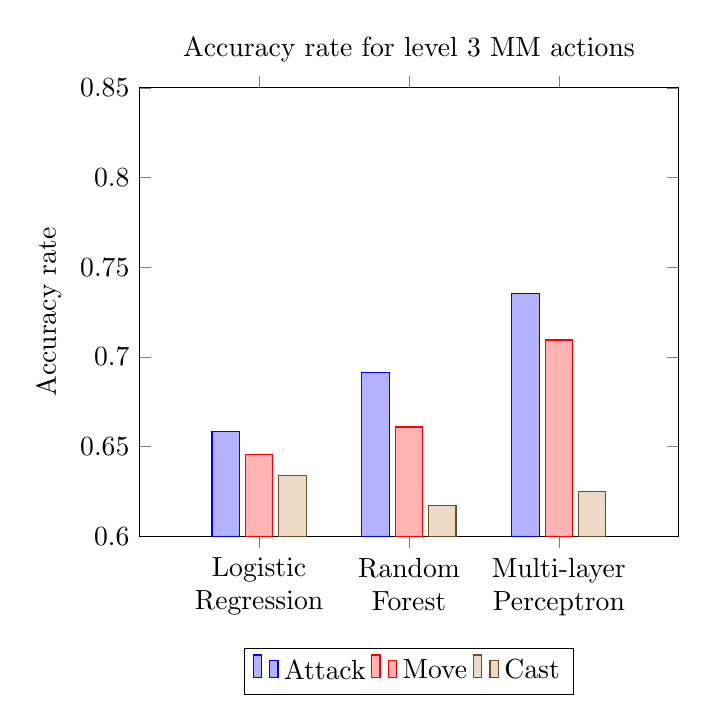
\begin{tikzpicture}
\newaxis{Accuracy rate for level 3 MM actions}{Accuracy rate}{0.6}{0.85}

\addplot coordinates {(Logistic Regression,0.6586) (Random Forest,0.6915) (Multi-layer Perceptron,0.7355)};
\addplot coordinates {(Logistic Regression,0.6457) (Random Forest,0.6609) (Multi-layer Perceptron,0.7094)};
\addplot coordinates {(Logistic Regression,0.6339) (Random Forest,0.6173) (Multi-layer Perceptron,0.6248)};
\legend{Attack,Move,Cast}

\end{axis}
\end{tikzpicture}
\end{subfigure}
\hspace{\fill}
\begin{subfigure}{0.45\textwidth}
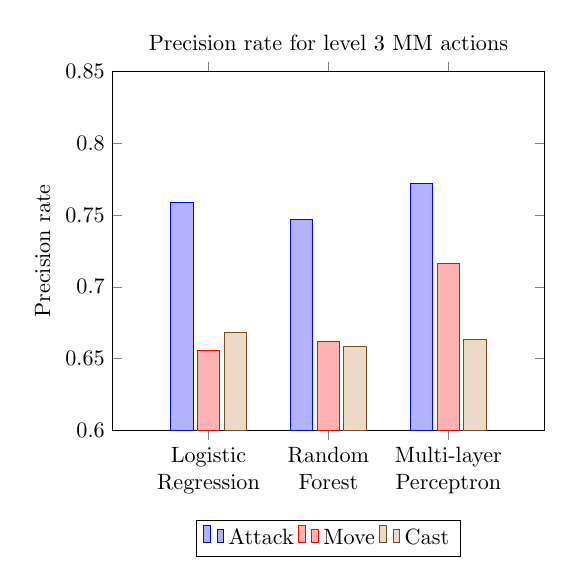
\begin{tikzpicture}[scale=0.8]
\newaxis{Precision rate for level 3 MM actions}{Precision rate}{0.6}{0.85}

\addplot coordinates {(Logistic Regression,0.759) (Random Forest,0.747) (Multi-layer Perceptron,0.7719)};
\addplot coordinates {(Logistic Regression,0.65524) (Random Forest,0.6618) (Multi-layer Perceptron,0.7165)};
\addplot coordinates {(Logistic Regression,0.6683) (Random Forest,0.6582) (Multi-layer Perceptron,0.6633)};
\legend{Attack,Move,Cast}

\end{axis}
\end{tikzpicture}
\end{subfigure}
\hspace{\fill}
\begin{subfigure}{0.45\textwidth}
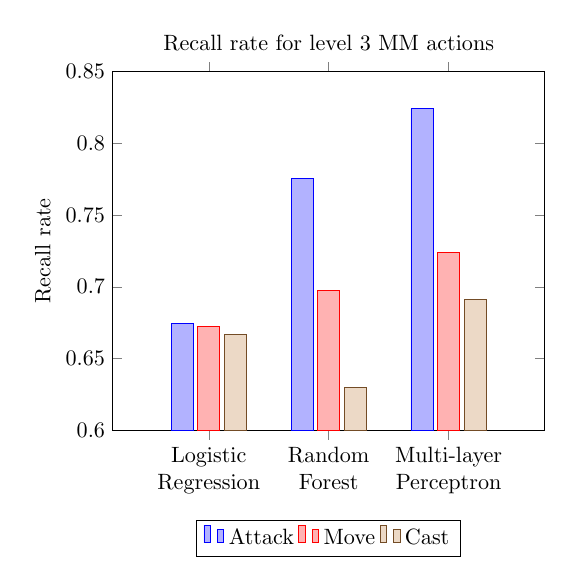
\begin{tikzpicture}[scale=0.8]
\newaxis{Recall rate for level 3 MM actions}{Recall rate}{0.6}{0.85}
\addplot coordinates {(Logistic Regression,0.6747) (Random Forest,0.7754) (Multi-layer Perceptron,0.8243)};
\addplot coordinates {(Logistic Regression,0.672) (Random Forest,0.6975) (Multi-layer Perceptron,0.7239)};
\addplot coordinates {(Logistic Regression,0.6665) (Random Forest,0.6301) (Multi-layer Perceptron,0.6909)};
\legend{Attack,Move,Cast}
\end{axis}
\end{tikzpicture}
\end{subfigure}
\caption{Classification rates using only mouse movement features.}
\label{fig:move-results}
\end{figure}

\subsubsection{Movements in each game}\label{sbsec:game-classification}

\begin{figure}[H]
\centering
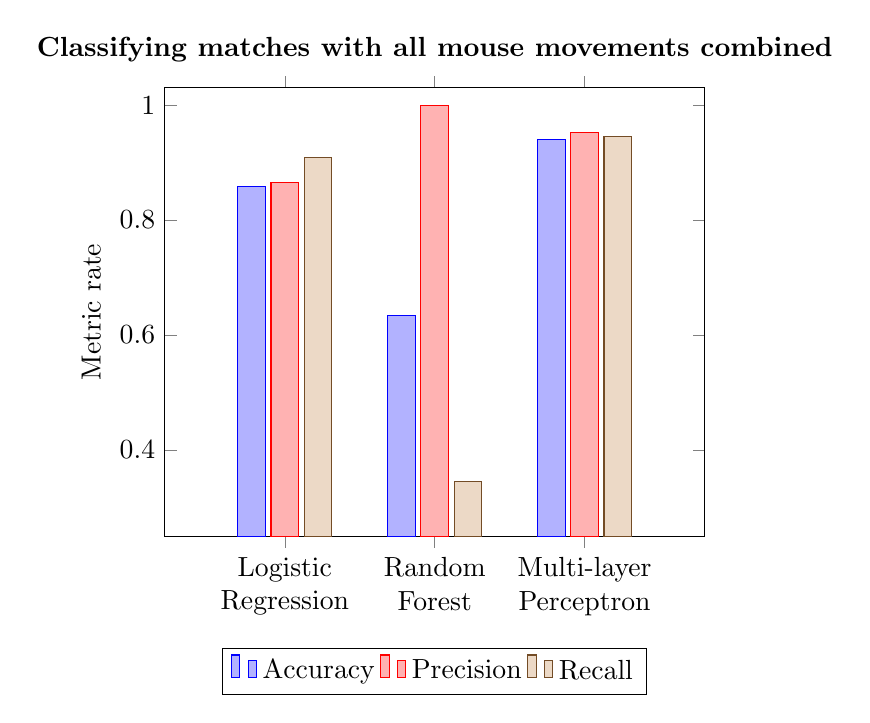
\begin{tikzpicture}
\newaxis{\textbf{Classifying matches with all mouse movements combined}}{Metric rate}{0.25}{1.03}

\addplot coordinates {(Logistic Regression,0.8589) (Random Forest,0.6347) (Multi-layer Perceptron,0.93947)};
\addplot coordinates {(Logistic Regression,0.8651) (Random Forest,1.0) (Multi-layer Perceptron,0.95256)};
\addplot coordinates {(Logistic Regression,0.909) (Random Forest,0.34545) (Multi-layer Perceptron,0.94545)};
\legend{Accuracy,Precision,Recall}

\end{axis}
\end{tikzpicture}
\caption{Training results of classifying each game. Note that the size of the dataset is reduced significantly compared to the previous classification approach because there are only a small number of games.}
\end{figure}

Recall that from \ref{fig:game-classifier-difference} that the three models are used only each type of mouse action, not the combination step, which remains the same. 

It can be seen that the logistic regression and multi-layer perceptron perform similarly well. 

% Logistic regression is a linear model, suggesting linear relation between the player and the mouse movement data

% Random forest gets perfect precision but low recall, hence likely predicting a very few positive results (shown by low recall), but always get the positive prediction correct (perfect precision)




\subsection{Game statistic features}

\subsection{Itemisation features}

\subsubsection{Hashed encoding}

\subsubsection{One-hot encoding}

\subsubsection{Starting items only}

\subsubsection{Boots only}


\subsection{Combining features}

% mouse and stats

% mouse and items

% stats and items

% mouse and stats and items

\end{document}
